\documentclass[tikz,border=8pt]{standalone}
\usetikzlibrary{arrows.meta,positioning}
\begin{document}
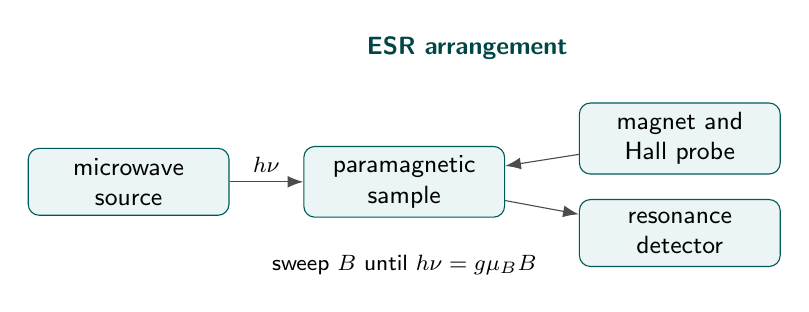
\begin{tikzpicture}[box/.style={draw=teal!70!black,fill=teal!8,rounded corners,minimum width=2.55cm,minimum height=.85cm,align=center,font=\sffamily\small},a/.style={-{Latex[length=2mm]},draw=black!70}]
\node[font=\sffamily\bfseries\small,text=teal!55!black] at (0,1.7) {ESR arrangement};
\node[box] (source) at (-4.3,0) {microwave\\source};
\node[box] (sample) at (-.8,0) {paramagnetic\\sample};
\node[box] (field) at (2.7,.55) {magnet and\\Hall probe};
\node[box] (detector) at (2.7,-.65) {resonance\\detector};
\draw[a] (source)--node[above,font=\sffamily\footnotesize]{$h\nu$} (sample);
\draw[a] (field)--(sample); \draw[a] (sample)--(detector);
\node[font=\sffamily\footnotesize] at (-.8,-1.05) {sweep $B$ until $h\nu=g\mu_BB$};
\end{tikzpicture}
\end{document}
